\chapter{Rapportens struktur} \label{metode}
Denne rapport tager udgangspunkt i metoden for en medicinsk teknologi vurdering (MTV), hvor en medicinsk problemstilling analyseres \citep{mtvhaandbog}. Yderligere er rapporten udarbejdet som et semesterprojekt på Aalborg Universitet, hvorfor den også tager udgangspunkt i problembaseret læring, hvor der opstilles et initierende problem, laves en problemanalyse og en problemformulering, der forsøges at besvare. 


\begin{figure}[H]
	\centering
	\includegraphics[width=0.5\textwidth]{figures/metodemodel}
	\caption{Model for den brugte metode i projektet.}
	\label{fig:metodemodel}
\end{figure}

\noindent
Som illustreret på \autoref{fig:metodemodel}, starter projektet bredt med et initierende problem, som analyseres og afgrænses i en problemformulering. Denne problemformulering forsøges besvaret gennem MTV-analyserne. 

MTV-analyserne belyser forskellige aspekter af teknologien ved at inddele MTV'en i fire områder: teknologi, patient, organisation og økonomi. %Der vælges at lægge mere vægt på udvalgte områder af MTV'en, da nogle af områderne er mere relevante for besvarelsen af problemformuleringen end andre.  

Hvert område vil have et tilhørende metodeafsnit til at beskrive, hvilke analysemetoder og fokuserende spørgsmål der bruges, og som er relevante for at kunne besvare den opstilled problemformulering. Den information som er nødvendig for at kunne besvare de fire MTV områder er i høj grad præget at eksisterende viden som er fundet ved at gennemføre en systematisk informationssøgning med udgangspunkt i de fire MTV områder. Metoden for informationssøgning beskrives yderligere i \autoref{sec:metode_soeg}. Ud over en systematisk informationssøgning indsamles information og data ved at udføre relevante observationer som kan være relevante for besvarelsen af visse MTV områder. Disse observationer ses især relevante på de områder hvor den eksisterende viden ikke har været tilstrækkelig for at kunne besvare de fokuserede spørgsmål under MTV analyserne.
%Måske en kilde til MTV bogen? :)

I syntesen vil de fire MTV-områder blive diskuteret, og der vil være en samlet konklusion på problemformuleringen ud fra delkonklusionerne i de fire MTV-analyser. 

\chapter{MTV-analyse}
Følgende kapitel beskriver de anvendte metoder i henholdsvis teknologi-, patient-, organisations- og økonomianalysen. Endvidere vil MTV-spørgsmålene til hver analyse fremgå. 

\section{Teknologi}\label{sec:metode_tek}
Teknologiafsnittet er opstillet ud fra en række MTV-spørgsmål, som vil beskrive teknologien og redegøre for og vurdere, hvilke teknologiske krav, Fitbit Flex skal opfylde for at kunne benyttes til at måle aktivitetsniveau hos hypertensive patienter. 
Foruden en tilpasset litteratursøgning ved brug af søgeprotokol, foretages beskrivelse af teknologien ud fra observationer ved anvendelse af software, der er relateret til teknologien.   
Herudover vil det blive undersøgt, hvilke effekter anvendelse af Fitbit Flex har på patientens sygdom.
 
\noindent
Dette giver anledning til følgende MTV-spørgsmål: 
\subsection{MTV-spørgsmål}
\begin{itemize}
\item Hvordan fungerer Fitbit Flex, og hvordan kan dette anvendes, således at en almen praktiserende læge får dokumenteret patientens aktivitetsniveau?
\item Repræsenterer Fitbit Flex den fysiske aktivitet tilstrækkeligt, til at data kan anvendes af praktiserende læger til vurdering af patientens fysiske aktivitetsniveau?
\end{itemize}

\section{Patient}\label{sec:metode_pat}
Til analyse af patienten og hvordan teknologien påvirker denne, anvendes \autoref{fig:patientaspekter}. Her analyseres sociale forhold, kommunikative forhold, økonomiske forhold, individuelle forhold og etiske forhold, samt sammenspillet mellem disse. I forhold til Fitbit Flex lægges der i denne analyse vægt på sociale forhold, herunder hvordan denne teknologi påvirker patientens arbejds- og uddannelsesliv, familie og livskvalitet, individuelle forhold, herunder hvordan patienten oplever teknologien, kommunikative forhold, samt etiske forhold, herunder risiko for misbrug af personlige data. 


\begin{figure}[H]
\centering
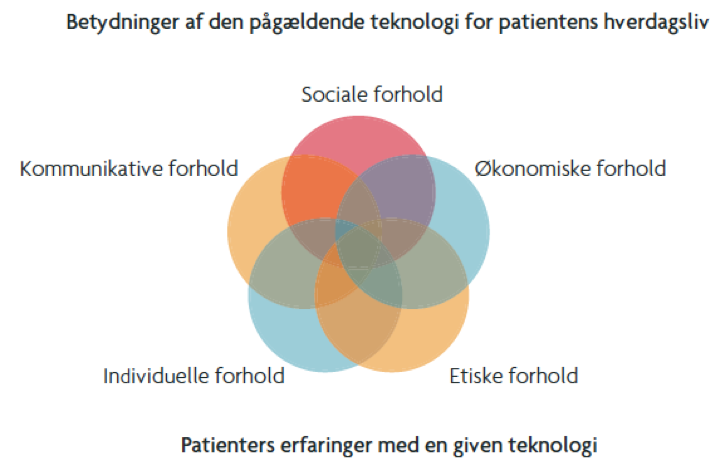
\includegraphics[width=0.8\textwidth]{figures/patientaspekter}
\caption{Patient-aspekter \citep{mtvhaandbog}.}
\label{fig:patientaspekter}
\end{figure}

\noindent
Dette giver anledning til følgende MTV-spørgsmål: 

\subsection{MTV-spørgsmål}
\begin{itemize}
\item Skal der være bestemte kriterier opfyldt for at patienten kan få udleveret en Fitbit Flex?
\item Er teknologien brugervenlig og motiverer den patienten til at få en mere aktiv hverdag?
\item Hvordan påvirker teknologien patienternes individuelle og sociale forhold i dagligdagen?
\item Hvor stor en andel af patienter oplever en positiv virkning ved anvendelse af teknologien, hvad er tidshorisonten for denne virkning, og hvad spiller en rolle for at teknologien giver et succesfuldt forløb?
\item Er der nogle etiske aspekter ved at monitorere patientens aktivitet, i så fald hvilke dilemmaer opstår heraf?
\end{itemize} 

\section{Organisation}\label{sec:metode_org}
Det ønskes at undersøge de organisatoriske forudsætninger samt mulige konsekvenser ved implementering af Fitbit Flex til monitorering af aktivitet i den primære sektor. Undersøgelsen tager udgangspunkt i den modificerede Leavitt organisationsmodel der ses af \autoref{fig:leavittmodel}, for at analysere konsekvenserne af en eventuel ændring i organisationen. Leavitts modificerede organisationsmodel benyttes, da denne tager højde for omgivelsernes påvirkning på teknologi, aktører, opgaver, struktur, disses indbyrdes påvirkning og påvirkning på omgivelserne. 
Teknologi omhandler arbejdsprocesser, procedurer og rutiner, i relation til teknologien.  
Aktører er de ansatte i organisationen, og deres holdninger og ekspertise i relation til organisationens opgaveløsninger. 
Opgaver dækker over de opgavetyper som organisationen forsøger at løse. 
Struktur omhandler formelle mønstre i organisationen, som arbejdsdeling og formalisering.  
Omgivelser er udvalgte interessenter, der er relevante i forhold til de organisatoriske ændringer. 

\begin{figure}[H]
\centering
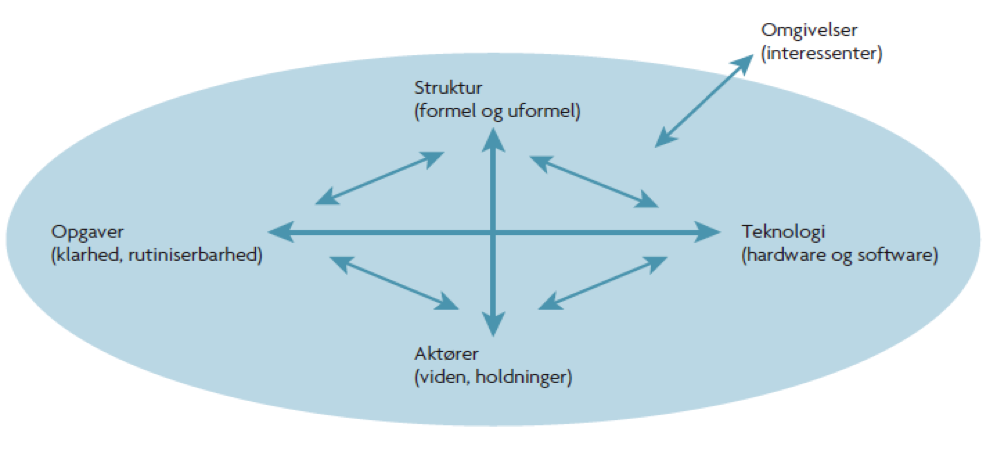
\includegraphics[width=0.9\textwidth]{figures/leavitt}
\caption{Leavitts modificerede organisationsmodel. Pilen mellem de forskellige områder betegner sammenspillet mellem dem. Dertil står omgivelser uden for de andre fire områder, da dette betgener hvem der har interesse for de organisatoriske ændringer der vil forekomme \citep{mtvhaandbog}.}
\label{fig:leavittmodel}
\end{figure}
\noindent
Dette giver anledning til følgende MTV-spørgsmål:

\subsection{MTV-spørgsmål}
\begin{itemize}
\item Hvordan passer Fitbit Flex i den primære sundhedssektor? 
\item Hvilke krav vil implementeringen stille til alment praktiserende læger, og hvem skal stå for en eventuel efteruddannelse? 
\item  Hvordan vil patientfordelingen mellem den primære og sekundære sundhedssektor blive påvirket, og hvad vil en ændring i arbejdsfordelingen medføre?
\end{itemize}

\section{Økonomi}\label{sec:metode_oeko}
I økonomianalysen undersøges mulige omkostninger, der kan forekomme ved implementering og anvendelse af Fitbit Flex som monitoreringsenhed for aktivitet til brug i almen praksis.
Ligeledes undersøges omkostninger for den nuværende monitoreringsmetode, samt hvilke økonomiske konsekvenser, der forekommer, når patienten ikke dyrker den anbefalede mængde motion.
Der vil derfor fremhæves mulige sundhedsmæssige resultater som følge af implementeringen af Fitbit Flex, i forhold til udgifterne dertil, uden at lave en egentlig cost-utility analyse, da de benyttede værdier er estimerede. 
Disse estimerede værdier i dette afsnit er baseret på udregninger ud fra funden litteratur omkring sundhedsøkonomi.

\noindent
Dette giver anledning til følgende MTV-spørgsmål: 

\subsection{MTV-spørgsmål}
 
\begin{itemize}
\item Hvad er omkostningerne ved nuværende monitoreringsmetode, samt konsekvenserne ved utilstrækkelig aktivitetsydelse? 
\item Hvilke omkostninger er forbundet med brug af Fitbit Flex til patienter med hypertension, og hvad er den økonomiske konsekvens af dette, hvis brug af aktivitetsarmbånd resulterer i et øget antal kvalitetsjusterede leveår?
\end{itemize}


%  Søgeprotokollen findes i \autoref{app:soegeprotokol}.